%==========================================================================

\begin{frame}[fragile]

  {\Huge General Enhancements}

  \vspace{10pt}

\end{frame}

%==========================================================================

% Examples

% note: always keep the [fragile] for your frames!

%\begin{frame}[fragile]{Example list}
%  \begin{itemize}
%      \item Item 1
%      \item Item 2 with some \texttt{code}
%      \begin{itemize}
%        \item Sub-item 2.1
%        \item Sub-item 2.2
%      \end{itemize}
%  \end{itemize}
%\end{frame}

%\begin{frame}[fragile]{Example code}
%    \begin{code}[keywords={std}]
%        #include <iostream>
%        
%        int main() {
%            std::cout << "hello world\n";
%        }
%    \end{code}
%\end{frame}

%\begin{frame}[fragile]{Example table}
%    \begin{center}
%        \begin{tabular}{l|l}
%            a & b \\\hline
%            c & d
%        \end{tabular}
%    \end{center}
%\end{frame}

%==========================================================================

\begin{frame}[fragile]{Fix a warning from kokkos\_check}
 \begin{itemize}
    \item \texttt{kokkos\_check}: Check at configure time that Kokkos was built with the requested backends and target architectures.
    \item Fix a warning when a user calls the cmake function \texttt{kokkos\_check} from a \texttt{<PackageName>Config.cmake} "Find Module" file
    {\tiny \begin{verbatim}
CMake Warning (dev) at /usr/share/cmake-3.22/Modules/FindPackageHandleStandardArgs.cmake:438 (message):
  The package name passed to `find_package_handle_standard_args`
  (Kokkos_DEVICES) does not match the name of the calling package (SomePackage).
  This can lead to problems in calling code that expects `find_package`
  result variables (e.g., `_FOUND`) to follow a certain pattern.
Call Stack (most recent call first):
  ... /kokkos/lib/cmake/Kokkos/KokkosConfigCommon.cmake:110 (find_package_handle_standard_args)
  ...
This warning is for project developers.  Use -Wno-dev to suppress it.
    \end{verbatim}}
 \end{itemize}
\end{frame}

\begin{frame}[fragile]{\texttt{inclusive\_scan} performance improvements}
  With the Cuda and HIP backends, \texttt{Kokkos::Experimental::inclusive\_scan} now calls the vendor versions in Thrust
  \begin{itemize}
     \item The vendor versions are up to 3x faster than the \texttt{Kokkos::parallel\_scan}-based default implementation
     \item Thrust requires \texttt{Kokkos\_ENABLE\_ROCTHRUST} to be \texttt{ON} (which is the default)
     \item Approximately 1.5-3x speed up (V100, MI300A)
  \end{itemize}
\end{frame}

\begin{frame}[fragile]{Reduce tooling interface overhead}
  Reduced the overhead of Kokkos tools related checks
  \begin{itemize}
      \item Store the information whether Kokkos tools are enabled after each modification to the tools' callbacks
      \item Previously, this value was recomputed for every event (\texttt{parallel\_for}, \texttt{fence}, etc.)
      \item Most noticeable in small serial kernels (around 100 elements)
      \item Reduction of launch time of approximately 10ns (About the time to increment 100 elements in a kernel) on CPU
  \end{itemize}
\end{frame}

%==========================================================================
\begin{frame}[fragile]{SIMD reductions and compound assignments}
  Added reductions and remaining compound assignments to Kokkos SIMD

  \begin{itemize}
    \item \texttt{basic\_simd\& operator/=(basic\_simd\&, U\&\&)}
    \item \texttt{basic\_simd\& operator>>=(basic\_simd\&, U\&\&)}
    \item \texttt{basic\_simd\& operator<<=(basic\_simd\&, U\&\&)}
  \end{itemize}

  \vspace{5pt}
  
  \begin{itemize}
    \item \texttt{T reduce\_min(const basic\_simd\& x)}
    \item \texttt{T reduce\_max(const basic\_simd\& x)}
    \item \texttt{T reduce(const basic\_simd\& x, const mask\_type\& mask, T identity\_element, BinaryOperation binary\_op)}
      \begin{itemize}
        \item Supported binary operations are: std::plus, std::multiplies, std::bit\_and, std::bit\_or and std::bit\_xor
        \item std::plus is used if binary op is not specified
      \end{itemize}
  \end{itemize}

\end{frame}
%==========================================================================
\begin{frame}[fragile]{Performance of algorithms}

  \begin{itemize}
    \item In Kokkos 4.5, we fixed a performance bug in \texttt{Kokkos::sort}
    \item Root cause is in an implementation detail in \texttt{RandomAccessIterator}
  \end{itemize}

  \vspace{10pt}

  \begin{itemize}
    \item In Kokkos 4.6 the root cause is fixed
    \item Fixes all algorithms that rely on \texttt{RandomAccessIterator} (e.g. sort,search,etc.)
  \end{itemize}

\end{frame}
%==========================================================================
\begin{frame}[fragile]{Performance of \texttt{search}}
\begin{center}
\textbf{Improvement dependent on algorithm and hardware!}
\end{center}

  \begin{center}
    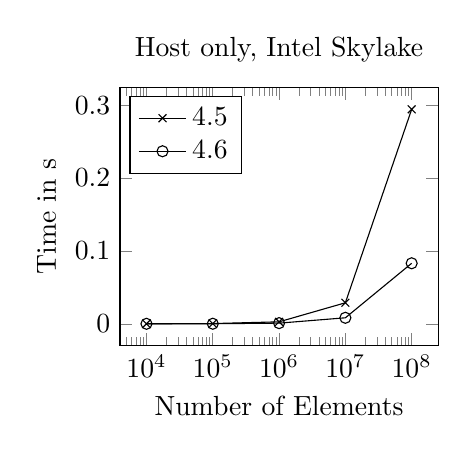
\begin{tikzpicture}
	\begin{axis}[
    title={Host only, Intel Skylake},
    legend pos=north west,
    xmode=log,
    height=0.4\textwidth,
		xlabel=Number of Elements,
    ylabel=Time in s]
	\addplot[mark=x] coordinates {
    (10000,3.0119e-05)
    (100000,0.000321003)
    (1000000,0.00270167)
    (10000000,0.0288293)
    (100000000,0.294202)
	};

	\addplot[mark=o] coordinates {
    (10000,8.57e-06)
    (100000,8.7155e-05)
    (1000000,0.000909428)
    (10000000,0.00823764)
    (100000000,0.0830087)
	};
  \legend{4.5,4.6}
	\end{axis}
\end{tikzpicture}

  \end{center}

\end{frame}
%==========================================================================
\begin{frame}[fragile]{Print support for system allocated memory}
  \texttt{print\_configuration} outputs if system allocated memory is accessible on GPU
  \begin{center}
    \textbf{No guarantees about the print format!}
  \end{center}

  \vspace{5pt}

  \begin{center}
    Example output for MI300A with HIP backend
  \end{center}
  \begin{code}
    XNACK environment variable set: yes
    Kernel reports HMM module via `CONFIG_HMM_MIRROR=y` in `/boot/config`: yes
    Architecture capable of accessing system allocated memory: 1,
    System allows accessing system allocated memory on GPU: 1,
  \end{code}
    
\end{frame}
%==========================================================================
